%%%%%%%%%%%%%%%%%%%%%%%%%%%%%%%%%%%%%%%%%%%%%%%%%%%%%%%%%%%%%%%%%%%%%%%%%%%%%%%%
%Tutorial slides on Python.
%
% Author: FOSSEE 
% Copyright (c) 2009, FOSSEE, IIT Bombay
%%%%%%%%%%%%%%%%%%%%%%%%%%%%%%%%%%%%%%%%%%%%%%%%%%%%%%%%%%%%%%%%%%%%%%%%%%%%%%%%

\documentclass[14pt,compress]{beamer}
%\documentclass[draft]{beamer}
%\documentclass[compress,handout]{beamer}
%\usepackage{pgfpages} 
%\pgfpagesuselayout{2 on 1}[a4paper,border shrink=5mm]

% Modified from: generic-ornate-15min-45min.de.tex
\mode<presentation>
{
  \usetheme{Warsaw}
  \useoutertheme{infolines}
  \setbeamercovered{transparent}
}

\usepackage[english]{babel}
\usepackage[latin1]{inputenc}
%\usepackage{times}
\usepackage[T1]{fontenc}

% Taken from Fernando's slides.
\usepackage{ae,aecompl}
\usepackage{mathpazo,courier,euler}
\usepackage[scaled=.95]{helvet}

\definecolor{darkgreen}{rgb}{0,0.5,0}

\usepackage{listings}
\lstset{language=Python,
    basicstyle=\ttfamily\bfseries,
    commentstyle=\color{red}\itshape,
  stringstyle=\color{darkgreen},
  showstringspaces=false,
  keywordstyle=\color{blue}\bfseries}

%%%%%%%%%%%%%%%%%%%%%%%%%%%%%%%%%%%%%%%%%%%%%%%%%%%%%%%%%%%%%%%%%%%%%%
% Macros
\setbeamercolor{emphbar}{bg=blue!20, fg=black}
\newcommand{\emphbar}[1]
{\begin{beamercolorbox}[rounded=true]{emphbar} 
      {#1}
 \end{beamercolorbox}
}
\newcounter{time}
\setcounter{time}{0}
\newcommand{\inctime}[1]{\addtocounter{time}{#1}{\tiny \thetime\ m}}

\newcommand{\typ}[1]{\lstinline{#1}}

\newcommand{\kwrd}[1]{ \texttt{\textbf{\color{blue}{#1}}}  }

% Title page
\title{Python for Scientific Computing : Least Square Fit}

\author[FOSSEE] {FOSSEE}

\institute[IIT Bombay] {Department of Aerospace Engineering\\IIT Bombay}
\date{}

% DOCUMENT STARTS
\begin{document}

\begin{frame}
  \maketitle
\end{frame}

\begin{frame}
  \frametitle{About the Session}
  \begin{block}{Goal}
Finding least square fit of given data-set
  \end{block}
  \begin{block}{Checklist}
    \begin{itemize}
    \item pendulum.txt
  \end{itemize}
  \end{block}
\end{frame}

\begin{frame}[fragile]
  \frametitle{$L$ vs. $T^2$ - Scatter}
  \vspace{-0.15in}
  \begin{figure}
    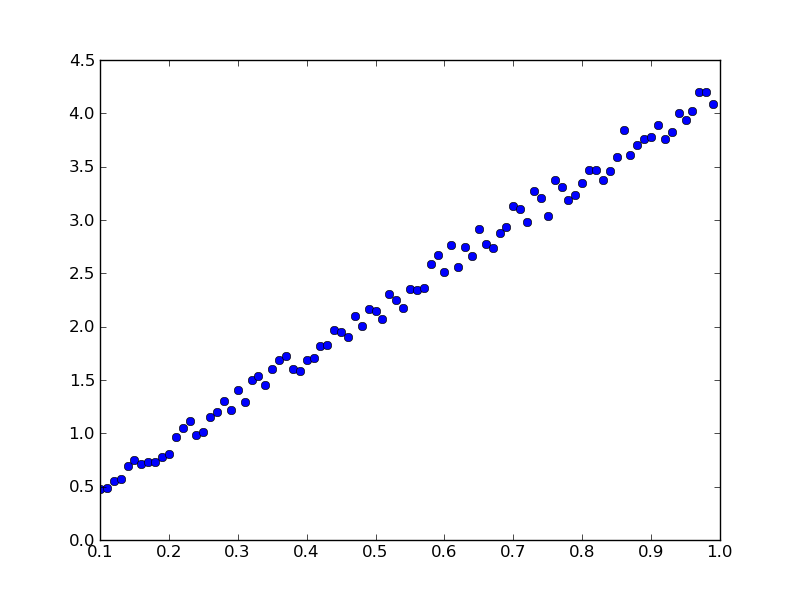
\includegraphics[width=4in]{data/L-Tsq-points}
  \end{figure}
\end{frame}

\begin{frame}[fragile]
  \frametitle{$L$ vs. $T^2$ - Line}
  \vspace{-0.15in}
  \begin{figure}
    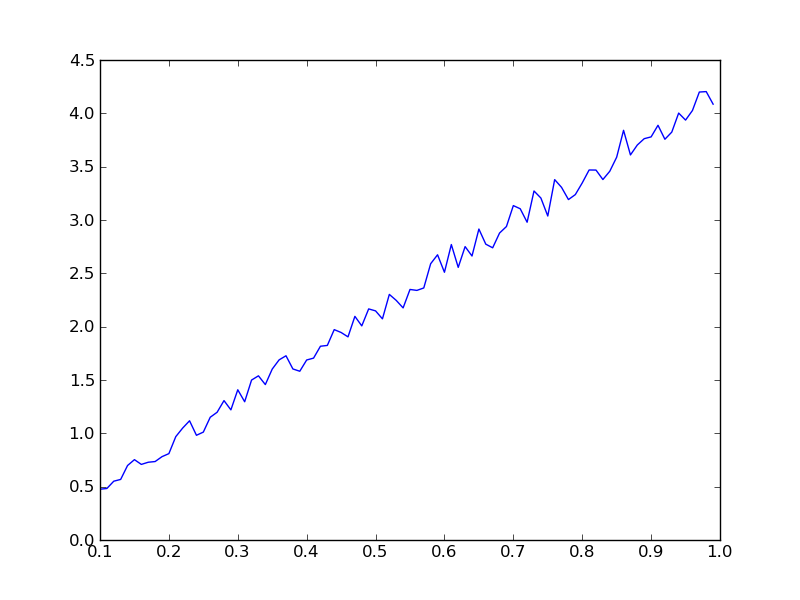
\includegraphics[width=4in]{data/L-Tsq-Line}
  \end{figure}
\end{frame}

\begin{frame}[fragile]
  \frametitle{$L$ vs. $T^2$ }
  \frametitle{$L$ vs. $T^2$ - Least Square Fit}
  \vspace{-0.15in}
  \begin{figure}
    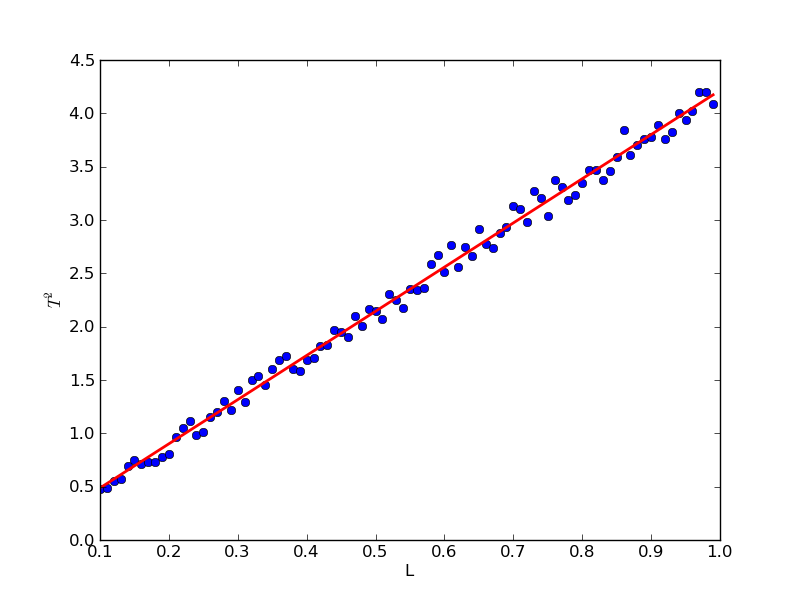
\includegraphics[width=4in]{data/least-sq-fit}
  \end{figure}
\end{frame}

\begin{frame}
  \frametitle{Least Square Fit Curve}
  \begin{center}
    \begin{itemize}
    \item $L \alpha T^2$
    \item Best Fit Curve $\rightarrow$ Linear
  \begin{itemize}
  \item Least Square Fit
  \end{itemize}
\item \typ{lstsq()} 
    \end{itemize}
  \end{center}
\end{frame}

\begin{frame}[fragile]
  \frametitle{\typ{lstsq}}
  \begin{itemize}
  \item We need to fit a line through points for the equation $T^2 = m \cdot L+c$
  \item In matrix form, the equation can be represented as $T_{sq} = A \cdot p$, where $T_{sq}$ is
  $\begin{bmatrix}
  T^2_1 \\
  T^2_2 \\
  \vdots\\
  T^2_N \\
  \end{bmatrix}$
, A is   
  $\begin{bmatrix}
  L_1 & 1 \\
  L_2 & 1 \\
  \vdots & \vdots\\
  L_N & 1 \\
  \end{bmatrix}$
  and p is 
  $\begin{bmatrix}
  m\\
  c\\
  \end{bmatrix}$
  \item We need to find $p$ to plot the line
  \end{itemize}
\end{frame}

\begin{frame}[fragile]
  \frametitle{Summary}
    Obtaining the least fit curve from a data set
\end{frame}

\begin{frame}
  \frametitle{Thank you!}  
  \begin{block}{}
  This session is part of \textcolor{blue}{FOSSEE} project funded by:
  \begin{center}
    \textcolor{blue}{NME through ICT from MHRD, Govt. of India}.
  \end{center}  
  \end{block}
\end{frame}

\end{document}
